\documentclass{article}

\usepackage{graphicx}
\usepackage{hyperref}

%----------------------------------------------------------------------------------------
%	ASSIGNMENT INFORMATION
%----------------------------------------------------------------------------------------

\title{CS5200: Homework \#1} % Title of the assignment

\author{Matthew Whitesides\\ \texttt{mbwxd4@mst.edu}} % Author name and email address

\date{\today} % University, school and/or department name(s) and a date

%----------------------------------------------------------------------------------------

\begin{document}

\maketitle % Print the title
 
\begin{enumerate}
  \item Signed statement on last page. 
  
  \item Question 2.
  \begin{enumerate}
    \item The age of the Earth is estimated at least 4.3 and commonly estimated at \textbf{4.54 billion years} old.

    \item The age of the Solar System is estimated between \textbf{4.53 and 4.58 billion years} old.

    \item The age of the Milky Way Galaxy is estimated at \textbf{11 to 13 billion years} old.

    \item The age of the universe is estimated at \textbf{10 to 15 billion years} old.
    \begin{itemize}
      \bibitem{usgs} 
      (Questions A - D): Dalrymple, G. Brent.
      \textit{The Age of the Earth}.
      \textit{\href{https://pubs.usgs.gov/gip/geotime/age.html}{https://pubs.usgs.gov/gip/geotime/age.html}}
      Stanford University Press, 492p, 1991.
    \end{itemize}

    \item The fate of the earth will probably be ended by our sun expanding into the earth in about 7 billion years putting the earth's lifespan at around \textbf{11 billion years} old.
    \begin{itemize}
      \bibitem{Ward} 
      Ward, Peter.
      \textit{The life and death of planet Earth}.      
      Holt, First edition, page 158, January 1, 2004.
    \end{itemize}

    \item There are many ways earth could become uninhabitable by humans however ignoring man-made disasters, and unplanned events such as an asteroid, the earth will naturally go through temperature cycles that would destroy civilization. A man killing ice age is hard to predict but could begin anywhere from \textbf{one to tens of thousands of years} from now, or millions, the last one was only 11 thousand years ago. Recent human activities have increased the climate decay and instability, and to preserve the climate as long as possible we would need to reduce our carbon emissions, and possibly on the survival of the species perspective would eventually need to figure out ways to massively heat or cool the earth survive natural global temperature cycles.
    \begin{itemize}
      \bibitem{Revkin} 
      Revkin, Andrew C.
      \textit{When Will the Next Ice Age Begin?}.
      \textit{\href{https://www.nytimes.com/2003/11/11/science/when-will-the-next-ice-age-begin.html}{https://www.nytimes.com/2003/11/11/science/when-will-the-next-ice-age-begin.html}}
      New York Times, Nov. 10, 2003, Section F, Page 6.
    \end{itemize}
    \begin{itemize}
      \bibitem{William} 
      Reville, William.
      \textit{How long will the human species survive on Earth?}.
      \textit{\href{https://www.irishtimes.com/news/science/how-long-will-the-human-species-survive-on-earth-1.2885564}{https://www.irishtimes.com/news/science/how-long-will-the-human-species-survive-on-earth-1.2885564}}
      Thu, Dec 8, 2016.
    \end{itemize}

    \item The estimated lifespan of the solar system will be about \textbf{11 billion years}. In around five billion years from now, the sun will enter a red giant phase and slowly expand outward for another billion years before exhausting all its energy.
    \begin{itemize}
      \bibitem{Redd} 
      Redd, Nola Taylor.
      \textit{Red Giant Stars: Facts, Definition and the Future of the Sun}.
      Schröder, Connon Smith, R. (2008).
    \end{itemize}

    \item There are many theories about how the universe will end but a commonly used one is related to heat death. In anywhere from \textbf{1 to 100 trillion years}, there will not be enough matter/energy for stars to form and the universe will contain mainly black holes which themselves will disappear eventually.
    \begin{itemize}
      \bibitem{Yun} 
      Wang, Yun.
      \textit{RCurrent observational constraints on cosmic doomsday}.
      Journal of Cosmology and Astro-Particle Physics. 2004 (12)
    \end{itemize}

    \item If there are 31536000 seconds in a year then (($2^{64}$ - 1) / 31536000) is equal to about \textbf{585 billion years} wich if we go with the lower estimate of the universe lifespan is around \textbf{59\%}.
  \end{enumerate}

  \item Question 3.
  \begin{enumerate}
    \item 
  \end{enumerate}

\end{enumerate}

\pagebreak

\begin{figure}
  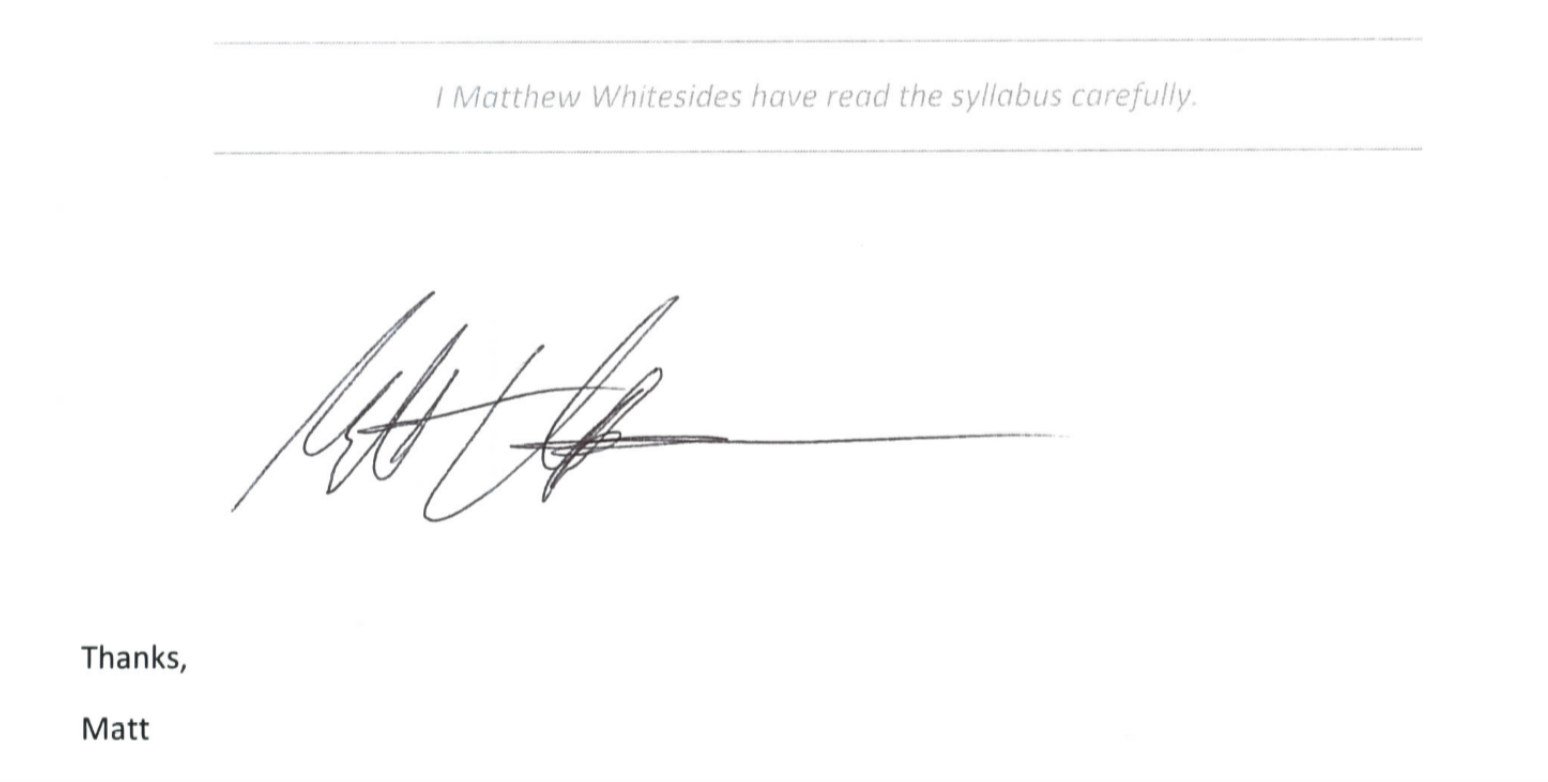
\includegraphics[width=\linewidth]{Statement.png}
  \label{fig:Statement}
\end{figure}

\end{document}
